\documentclass[hidelinks, 12pt, letterpaper]{article}
\usepackage[margins=0.25in]{geometry}
\usepackage[dvipsnames]{xcolor}
\usepackage{amsmath}
\usepackage{tikz}
\usepackage{tkz-euclide}
\usepackage[unicode]{hyperref}
\usepackage[all]{hypcap}
\usepackage{fancyhdr}

\usetikzlibrary{angles,calc, decorations.pathreplacing}

\definecolor{carminered}{rgb}{1.0, 0.0, 0.22}
\definecolor{capri}{rgb}{0.0, 0.75, 1.0}
\definecolor{brightlavender}{rgb}{0.75, 0.58, 0.89}

\title{\textbf{Lab 1:  Introduction to Motion Detectors}\\PHYS 211L}
\author{H. Ryott Glayzer\\Collaborators: Ruccus and others}
\date{\today}
\begin{document}
\hypersetup{bookmarksnumbered=true,}
%\pagecolor{black}
%\color{white}
\maketitle

\begin{large}
\tableofcontents
\end{large}%
\pagebreak

\section{Introduction}
In this lab, students utilize ultrasonic motion detectors,
the CAPSTONE software, and Microsoft Excel to explore 
experimental setup, data acquisition, and basic data analysis.
The PASCO brand motion detectors provide data on position, velocity,
and acceleration relative to time.
This data is collected by students who utilize Microsoft Excel to 
analyze it.

The experiment involves students measuring the change in position,
relative to time, of a student both walking and running. 
Students will utilize this data to determine the speed of motion,
as well as the acceleration.
It is assumed that when walking, the student will have a constant velocity,
and the student will have a constant acceleration while running.
This is only approximately true, as students cannot rigidly control
their movements in order to perfectly align with these assumptions.

\section{Procedure}
For the first experiment, students will get the ultrasonic sensor and its 
software running.
Once it is running, a student will stand in front of the sensor, about a half 
of a meter away, and begin walking away from the detector once the `record' button 
is pressed on the software.
The student should walk a clear path of at least two meters.
After the student has finished, the group should ensure the data is reasonable and 
redo this part of the experiment if not.
The second part of the experiment is similar, but involves the student running
from a dead stop rather than walking.
Completely copying the Lab Manual word for word would be hell for my carpal tunnel.

The Lab Manual suggests analyzing the data in excel using trend fitting.
However, I strayed from the exact procedure here and used python to fit my trends.
I also utilized the Chi-Square Goodness of Fit test, rather than the r-square
statistic, since the Chi-Square statistic test explores how well the data fits a 
model, rather than measuring the proportion of variation of the data itself.


\section{Data and Plots}
The raw data for this experiment is available as a CSV file that can be provided
upon request, the data is represented well by the following plots.
Typing out the data points in \LaTeX would be an exercise in futility.

The first plot shows the relationship between the walking student's position
and time, as well as the fit line for the data.
The student could not keep a perfectly steady pace, but that is expected 
for a human and is within the confines of error for this experiment.
The chi-square value in this plot confirms the null hypothesis. 
In other words, the regression fits the observed data well.

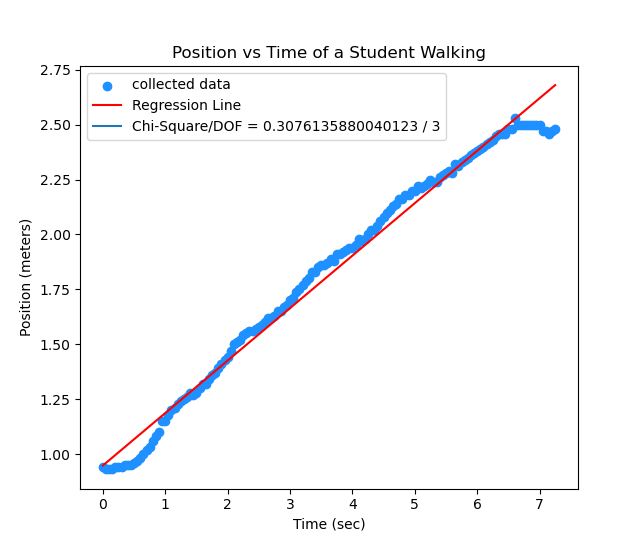
\includegraphics[width=0.9\linewidth]{walking-plot.png}

The second plot outlines the relationship between the running student's
position and time. 
A quadratic trend is observed, and the chi-square statistic indicates that
the quadratic model is a good fit for the data.

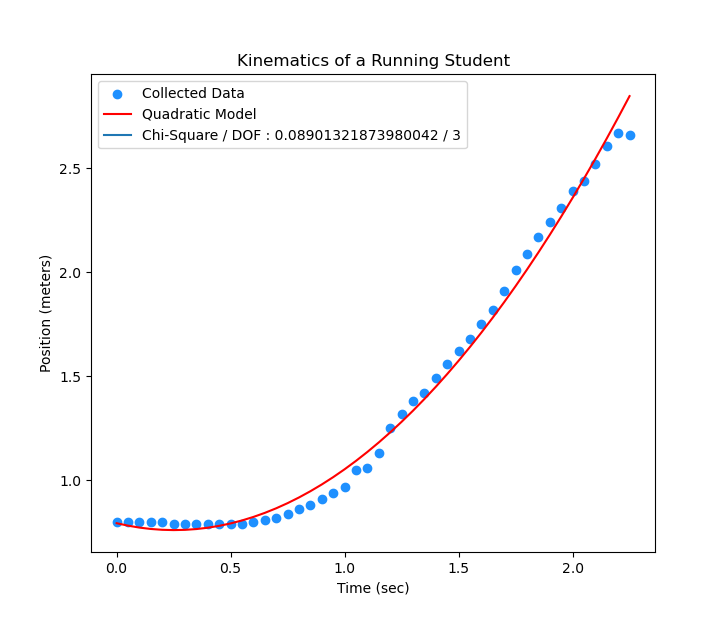
\includegraphics[width=0.9\linewidth]{run_plot.png}

Later, the Lab Manual asks students to find the average velocity,
as measured by the PASCO software.
When I performed this calculation,
I was surprised to see that the average acceleration was
apparently $0.064 \; m/s^2$.
Thus, I decided to investigate further.
I made a plot of kinematic values (acceleration, velocity, and position)
plotted with each other against time.
This helped me to understand that the data included many negative 
points of instantaneous acceleration, 
which skewed the data toward zero.

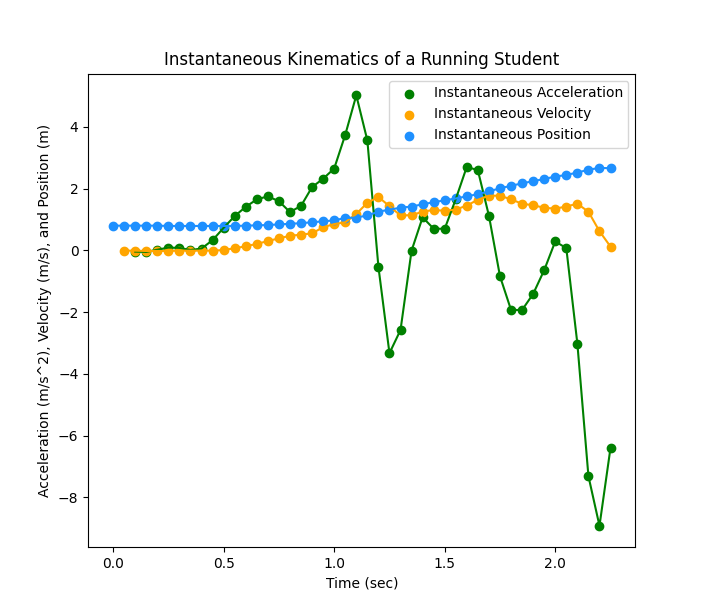
\includegraphics[width=0.9\textwidth]{running-comparison.png}

\section{Calculations}

The calculations that were performed to obtain this data are available
as a python file that will be provided.
I am not sure how to include this in a paper format other than 
simply printing out my code, as my only print statements are 
progress statements and debugging statements.

I utilized the linear regression model from scikit-learn, as well as
the quadratic regression model from scipy.stats. Degrees of freedom were
determined as (position + time + 1 = 3).
I created my own chi-square module:

\begin{verbatim}
# Exerpt from fit.py
# Copyright © 2024 H. Ryott Glayzer
# MIT License

def chiSquare(observed, expected):
    """Performs a chi squared goodness-of-fit test"""
    middleVal = []
    for i in range(len(observed)):
        value = ((observed[i] - expected[i])**2 / expected[i])
        middleVal.append(value)

    chiSquareStatistic = sum(middleVal)
    return chiSquareStatistic
\end{verbatim}

The output to \verb|STDOUT| from my code was as follows:

\begin{verbatim}
Walking Data Imported... 
Making time cuts in Walking Data... 
f(x)=[[0.23901054]]x+[0.94769639]
Deviation from Model for Walking Model: 0.0611050917013222
Importing Running Data... 
Making Time Cuts in Running Data
        2
0.5228 x - 0.2634 x + 0.7937
Deviation from Model for Quadratic Fit: 0.05380773460038573
Mean Acceleration: Time (s) Run #1               1.125000
Position (m) Run #1           1.389348
Velocity (m/s) Run #1         0.827556
Acceleration (m/s²) Run #1    0.064318
dtype: float64
\end{verbatim}  

The mean acceleration was found using the Pandas library's 
\verb|DataFrame.mean()| method, not dissimilar to the method described
for Excel.

\section{Error Analysis}
I find it difficult to quantify error in this experiment, as I do not have
a control or any knowledge of the tolerances or precision of the equipment used.
However, I am able to qualitatively describe the likely sources of error and 
how it would affect the data.
The ultrasonic sensors have been characterized as unreliable and touchy,
which would make it difficult to trust the precision of the data collected,
especially within the messy conditions that Phys I lab is performed in.
From a completely qualitative prospective, though, the level of precision necessary for our purposes is achieved.

However, looking at the fit itself,
and putting aside the systemic error calculations,
we find that the Chi-Square statistic is near zero for both
fit models, which would indicate that our model fits well, with relatively
low uncertainties.


\section{Results}
In this experiment, we found that Ruccus' walking is best represented
by the function 
\begin{equation}
    f(t) = 0.239t + 0.947 \pm 0.061, 
\end{equation}
where \textit{t} is time in seconds, and \textit{f(t)} is distance from the 
sensor in meters.
We also found that Ruccus' running is best represented by the function
\begin{equation}
    f(t) = 0.523t^{2} - 0.263t + 0.794 \pm 0.054, 
\end{equation}
also in respect to time and distance from the sensor.
The uncertainties presented here were obtained via
\begin{equation}
    \mu = \pm\sqrt{\frac{(f_{observed} - f_{expected})^{2}}{n}}.
\end{equation}

\section{Questions}
\subsection{Part 1, Question 1: Equation of Motion} 
After performing a data cut to include only the first walk away for 
simplicity in data analysis, the equation of motion for Ruccus walking
is 
\begin{equation}
    f(t) = 0.239t + 0.948,
\end{equation}
where 
$t$ represents time in seconds and $f(t)$ represents meters of distance.
\subsection{Part 1, Question 2: Velocity}
The student's velocity was $0.239 \; m/s$.

\subsection{Part 2, Question 1}
Utilizing the position vs. time formula, the acceleration is 
$1.046 \; m/s^{2}$, with the equation of motion being 
$f(t) = 0.523t^{2} - 0.263t + 0.794 $.

\subsection{Part 2, Question 2}
When utilizing quadratic regression,
I found an acceleration value of $1.046\; m/s^{2}$;
however, when simply averaging the instantaneous acceleration
data points that the average was surprisingly low: 
$0.064 \; m/s^2$.
I created a plot of acceleration vs. time (see Figure 3)
and found that there were many points of 
negative instantaneous acceleration.
There is a $93\%$ error between these acceleration values.



\section{Conclusions}
Overall, this experiment was subject to more variables
than we accounted for in our data-taking.
Humans have difficulty maintaining constant velocity,
as well as constant acceleration, unless we are dead and 
unmoving, with both values equaling zero.
For the precision necessary for a PHYS 211 exploration into
basic kinematics, our experiment was okay.
We were able to observe changes in velocity relating to 
acceleration, as well as changes in position relating to 
both velocity and acceleration.
We garnered firsthand experience with the frustrations
of utilizing outdated, worn-down equipment,
which will help prepare us for much of the rest of our
careers as  students.
The availability of control data, as well as better
quantifiable information on the detectors themselves
would have allowed for a more in-depth exploration 
of uncertainty and error propagation.
We found that Ruccus walks at a reasonably normal
pace, and is bad at keeping constant acceleration. 
Our exploration of basic kinematics yielded predictably
uninteresting results that precisely followed the laws
of physics.
We also came to understand the limitations posed by
ultrasonic sensors in regard to failures in obtaining 
correct data.
Finally, I was able to learn that many students practice 
bad data-taking habits. 
This was definitely an interesting lab.




\end{document}
